\documentclass[8pt,fleqn]{beamer}

%---------------------------------------------------------------
% Macros
% version 3 by Igor Ruiz-Agundez 2011
% version 2 by Jakob Suckale 2007
% version 1 by Harish Bhanderi 2002
%---------------------------------------------------------------

% This file contains macros that can be called up from connected TeX files
% It helps to summarise repeated code, e.g. figure insertion (see below).


%---------------------------------------------------------------
% MY COMMANDS
%---------------------------------------------------------------
%MY COMMANDS
\newcommand{\sub}[1]{\mbox{\scriptsize{#1}}}
\newcommand{\der}[2]{ \frac{ \partial #1 }{\partial #2} }
\newcommand{\dtot}[2]{ \frac{ d #1 }{d #2} }
\newcommand{\pr}[1]{ \left( #1 \right) }
\newcommand{\cor}[1]{ \left[ #1 \right] }
\newcommand{\lla}[1]{ \left\{ #1 \right\} }
\newcommand{\eq}[2]{\begin{equation} \label{#1} #2 \end{equation}}
\newcommand{\bds}[1]{\boldsymbol{ #1 }}
\newcommand{\oiint}{\displaystyle\bigcirc\!\!\!\!\!\!\!\!\int\!\!\!\!\!\int}
\newcommand{\mathsize}[2]{\mbox{\fontsize{#1}{#1}\selectfont $#2$}}
\newcommand{\sinc}[1]{\mbox{sinc}#1}

\newcommand{\cita}[1]{\textsuperscript{\tiny\cite{#1}}}
\newcommand{\ket}{\rangle}
\newcommand{\bra}{\langle}

\renewcommand{\listtablename}{Índice de tablas}
\renewcommand{\tablename}{Tabla}

\usepackage{color, colortbl}
%Celda de colores en tablas
\newcommand{\cellc}[1]{\multicolumn{1}{|>{\columncolor[rgb]{0.8, 0.8, 0.8}}c|}{#1}}

%---------------------------------------------------------------
% Figures
%---------------------------------------------------------------


% Makes the \InsertFig macro compatible both with one or two columns
\makeatletter
\newlength \figwidth
\if@twocolumn
  \setlength \figwidth {\columnwidth}
\else
  \setlength \figwidth {\textwidth}
\fi
\makeatother

% \InsertFig allows inserting figures
% Parameters
% 1 --> Filename
% 2 --> Label for referencing
% 3 --> Title describing the figure (caption)
% 4 --> Description of the figure
% 5 --> Figure width, range [0,1]. If parameter is left blank the figure size is not change
% 6 --> Any other option for \includegraphics
% Usage:
% \InsertFig{}{}{}{}{}{}
%
\newcommand{\InsertFig}[6]{%
	\ifthenelse{\isempty{#5}}%
	{% if #1 is empty
		\begin{figure}[htbp!]
		\centering
		\includegraphics[#6]{#1}%
		\caption{#3}{\textbf{#4}}
		\label{#2}
		\end{figure}    
	}
	{% if #1 is not empty
		\begin{figure}[htbp!]
		\centering
		\includegraphics[width=#5\figwidth,#6]{#1}%
		\caption{#3}{\textbf{#4}}
		\label{#2}
		\end{figure}
	}
}

%% Simple version of \InsertFig
%\newcommand{\InsertFig}[5]{
%  \begin{figure}[htbp]
%   	\centering
%    \includegraphics[width=#4\textwidth,#5]{#1}%
%    \caption{#3}
%    \label{#2}
%  \end{figure}
%}



% insert a centered figure with caption
% parameters 1:filename, 2:label, 3:title, 
\newcommand{\figuremacro}[3]{
	\begin{figure}[htbp]
		\centering
		\includegraphics[width=1\textwidth]{#1}
		\caption[#3]{\textbf{#3}}
		\label{#2}
	\end{figure}
}


% insert a centered figure with caption and description
% parameters 1:filename, 2:label, 3:title, 4:description
\newcommand{\figuremacroD}[4]{
	\begin{figure}[htbp]
		\centering
		\includegraphics[width=1\textwidth]{#1}
		\caption[#3]{\textbf{#3} - #4}
		\label{#2}
	\end{figure}
}

% insert a centered figure with caption and description AND WIDTH
% parameters 1:filename, 2:label, 3:title, 4:description, 5: textwidth
% textwidth 1 means as text, 0.5 means half the width of the text
\newcommand{\figuremacroDW}[5]{
	\begin{figure}[htbp]
		\centering
		\includegraphics[width=#5\textwidth]{#1}
		\caption[#3]{\textbf{#3} - #4}
		\label{#2}
	\end{figure}
}

% inserts a figure with wrapped around text; only suitable for NARROW figs
% o is for outside on a double paged document; others: l, r, i(inside)
% text and figure will each be half of the document width
% note: long captions often crash with adjacent content; take care
% in general: above 2 macro produce more reliable layout
\newcommand{\figuremacroN}[3]{
	\begin{wrapfigure}{o}{0.5\textwidth}
		\centering
		\includegraphics[width=0.48\textwidth]{#1}
		\caption[#2]{{\small\textbf{#2} - #3}}
		\label{#1}
	\end{wrapfigure}
}




% Estas definiciones son para el comando \InsertFigBox
\newlength{\anchoFigura}
\newlength{\anchoFloat}
\addtolength{\fboxsep}{2\fboxsep}
%\renewcommand{\capfont}{\normalfont\normalcolor\sffamily\small}
%\renewcommand{\caplabelfont}{\normalfont\normalcolor\sffamily\bfseries\small}

% El comando \InsertFigBox nos permite insertar figuras en un marco
% Los parametros son:
% 1 --> Fichero de la imagen
% 2 --> Etiqueta (label) para referencias
% 3 --> Texto a pie de imagen
% 4 -> Porcentaje del ancho de página que ocupará la figura (de 0 a 1)
% 5 --> Opciones que queramos pasarle al \includegraphics
\newcommand{\InsertFigBox}[5]{%
  \setlength{\anchoFloat}{#4\textwidth}%
  \addtolength{\anchoFloat}{-4\fboxsep}%
  \setlength{\anchoFigura}{\anchoFloat}%
  \begin{figure}%
    \begin{center}%
      \Ovalbox{%
        \begin{minipage}{\anchoFloat}%
          \begin{center}%
            \includegraphics[width=\anchoFigura,#5]{#1}%
            \caption{#3}%
            \label{#2}%
          \end{center}%
        \end{minipage}
      }%
    \end{center}%
  \end{figure}%
}



%---------------------------------------------------------------
% Misc
%---------------------------------------------------------------

% predefined commands by Harish
\newcommand{\PdfPsText}[2]{
  \ifpdf
     #1
  \else
     #2
  \fi
}


%---------------------------------------------------------------
% Locales
%---------------------------------------------------------------


%%
%% Para quitar traducciones raras (Cuadros)
%% A de usarse cada vez que se seleccione el idioma
%%
\newcommand{\MejorarTraducciones}{%
       \renewcommand{\listtablename}{Índice de tablas}
       \renewcommand{\tablename}{Tabla}
       \renewcommand{\lstlistingname}{Lista}
}%



%---------------------------------------------------------------
% Source code
%---------------------------------------------------------------


%%
%% Para escribir extractos de codigo
%%
%% Las tabulaciones se substituyen por dos espacios
%\fvset{tabsize=2}
%% Creamos un nuevo environment de fancyvrb para los ejemplos enmarcados
%\DefineVerbatimEnvironment{VerbEj}{BVerbatim}{fontsize=\small,samepage=true,commandchars=\\\{\}}
%% Colo de fondo
%\definecolor{grisfondo}{gray}{0.9}
%% Environment para extractos de codigo
%\newenvironment{codigo}%
%{\VerbatimEnvironment\begin{Sbox}\begin{VerbEj}}%
%{\end{VerbEj}\end{Sbox}\setlength{\fboxsep}{8pt}\begin{center}\fcolorbox{black}{grisfondo}{\TheSbox}\end{center}}
%
%% Otro formato más bonito para código fuente
%\newcommand{\codigofuente}[3]{%
%  \lstinputlisting[language=#1,caption={#2}]{#3}%
%}






\title{\textbf{The Place of the Milky Way and Andromeda in the Cosmic Web} \\ .\\ 
\small{\textbf{Author:} Sebastian Bustamante -- Universidad de Antioquia\\
\textbf{Advisor:} Jaime Forero -- Universidad de los Andes}
\author[Sebastian Bustamante]{}}
\institute[FACom]{}


\begin{document}
\justifying
%=========================================================================
%			TITLE PAGE
\begin{frame}
\titlepage
\end{frame}
%=========================================================================
%			VIDEO COSMIC WEB
\begin{frame}
\begin{tcolorbox}[colback=white!5,colframe=black!75!black,title=Cosmic Web]\centering

\

	\movie[]{\includegraphics[width=0.6\textwidth]{figures/Bolshoi_Frame.jpg}}{videos/Bolshoi_zoomed.mp4}
	
\

\end{tcolorbox}
\end{frame}
%=========================================================================
%			ZOOMED COSMIC WEB
\begin{frame}
\begin{tcolorbox}[colback=white!5,colframe=black!75!black,title=Cosmic Web]\centering

\

	\includegraphics[trim = 0mm 0mm 0mm 0mm, clip, width=0.6\textwidth]
	{./figures/Cosmic_Web_Zoomed.png}
	
\

\end{tcolorbox}
\end{frame}
%=========================================================================
%			ZOOMED COSMIC WEB
\begin{frame}
\begin{tcolorbox}[colback=white!5,colframe=black!75!black,title=Observed Cosmic Web (SDSS)]\centering
\

	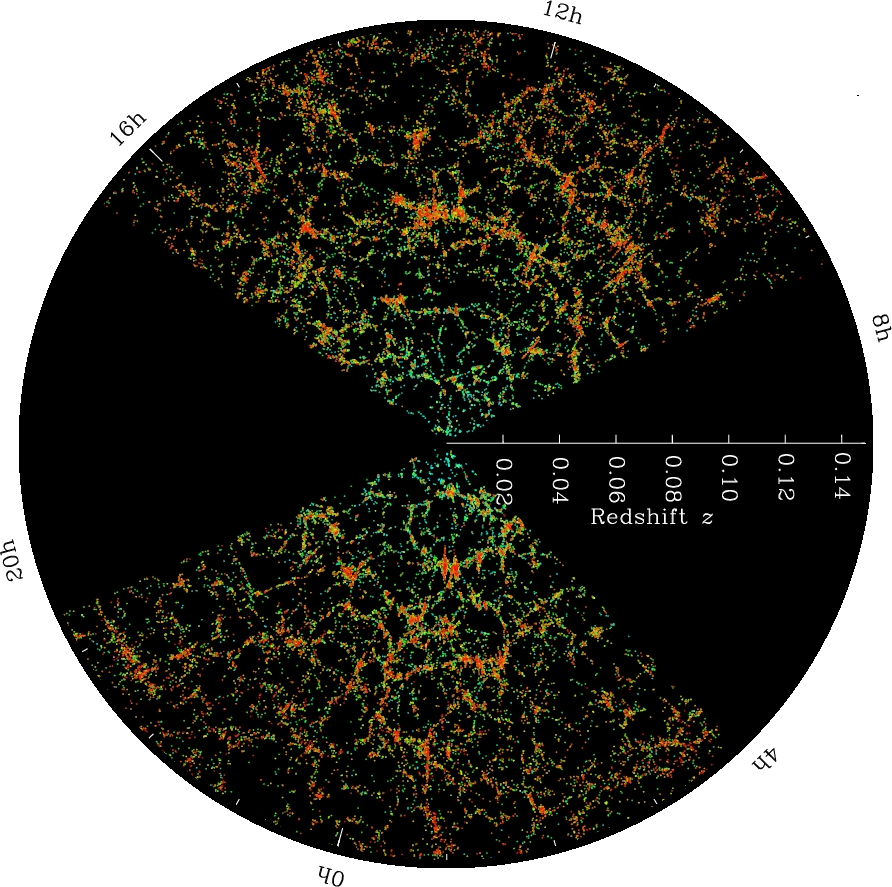
\includegraphics[trim = 0mm 0mm 0mm 0mm, clip, width=0.6\textwidth]
	{./figures/SDSS.png}
	
\

\end{tcolorbox}
\end{frame}
%=========================================================================
%			MOTIVATION (1.)
\begin{frame}
\begin{tcolorbox}[colback=white!5,colframe=black!75!black,title=Motivation]\justifying

	\begin{enumerate}
	\color{black}
	\item Quantify the structure of the Cosmic Web.
	\end{enumerate}

\end{tcolorbox}
\end{frame}
%=========================================================================
%			LOCAL GROUP (NO MARKED)
\begin{frame}
\begin{tcolorbox}[colback=white!5,colframe=black!75!black,title=Local Group]\justifying
\begin{figure}[htbp]
	\centering
	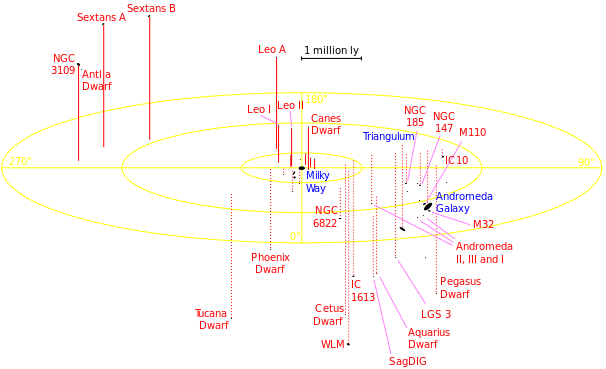
\includegraphics[trim = 0mm 0mm 0mm 50mm, clip, width=0.75\textwidth]
	{./figures/LocalGroup.png}
\end{figure}
\end{tcolorbox}
\end{frame}
%=========================================================================
%			LOCAL GROUP (MARKED)
\begin{frame}
\begin{tcolorbox}[colback=white!5,colframe=black!75!black,title=Local Group]\justifying
\begin{figure}[htbp]
	\centering
	\includegraphics[trim = 0mm 0mm 0mm 50mm, clip, width=0.75\textwidth]
	{./figures/LocalGroup_Marked.png}
\end{figure}
\end{tcolorbox}
\end{frame}
%=========================================================================
%			MOTIVATION (2.)
\begin{frame}
\begin{tcolorbox}[colback=white!5,colframe=black!75!black,title=Motivation]\justifying

	\begin{enumerate}
	\color{black}
	\item Quantify the structure of the Cosmic Web.
	\item Construct samples of LG-like systems in (unconstrained) cosmological 
	simulations.
	\end{enumerate}

\end{tcolorbox}
\end{frame}
%=========================================================================
%			LG'S IN COSMIC WEB
\begin{frame}
\begin{tcolorbox}[colback=white!5,colframe=black!75!black,title=Cosmic Web]\centering

\

	\includegraphics[trim = 0mm 0mm 0mm 0mm, clip, width=0.6\textwidth]
	{./figures/LG_Cosmic_Web.png}

\

\end{tcolorbox}
\end{frame}
%=========================================================================
%			MOTIVATION (3.)
\begin{frame}
\begin{tcolorbox}[colback=white,colframe=black!75!black,title=Motivation]\justifying
	
	\begin{enumerate}
	\color{black}
	\item Quantify the structure of the Cosmic Web.
	\item Construct samples of LG-like systems in (unconstrained) cosmological 
	simulations.
	\item Find possible effects of the local environment on the physical 
	properties of LG-like systems
	\item What is the most likely host environment of LG-like systems?
	\end{enumerate}

\end{tcolorbox}
\end{frame}
%=========================================================================
%			SIMULATIONS
\begin{frame}
\begin{tcolorbox}[colback=white!5,colframe=black!75!black,title=Simulations]\justifying
\begin{columns}
\column[t]{3cm}
	\begin{itemize}
	\color{black}
	\item \textbf{Unconstrained Simulation} 
	
	\textit{\textbf{(Bolshoi project)}}
	\begin{small}
	\begin{itemize}
	\color{black}
	\item $250 h^{-1}$Mpc
	\item $\Lambda$CDM
	\item WMAP7 \\
	\item $2048^{3}$ particles
	\item $1.35 \times 10^8$M$_{\odot}/h$	
	\end{itemize}
	\end{small}
	
	\vspace{.7cm}
	\item \textbf{Constrained Simulations} 
	
	\textbf{(CLUES project)}
	\begin{small}
	\begin{itemize}
	\color{black}
	\item $64 h^{-1}$Mpc
	\item $\Lambda$CDM
	\item WMAP7 \\
	\item $1024^{3}$ particles
	\item $1.83 \times 10^7$M$_{\odot}/h$	
	\end{itemize}
	\end{small}
	
	\end{itemize}
\column[t]{7cm}
	%\begin{center}
	\
	
	\includegraphics[trim = 5mm 5mm 5mm 5mm, clip, width=.5\textwidth]
	{./figures/Bolshoi_Simulation.pdf}
	
	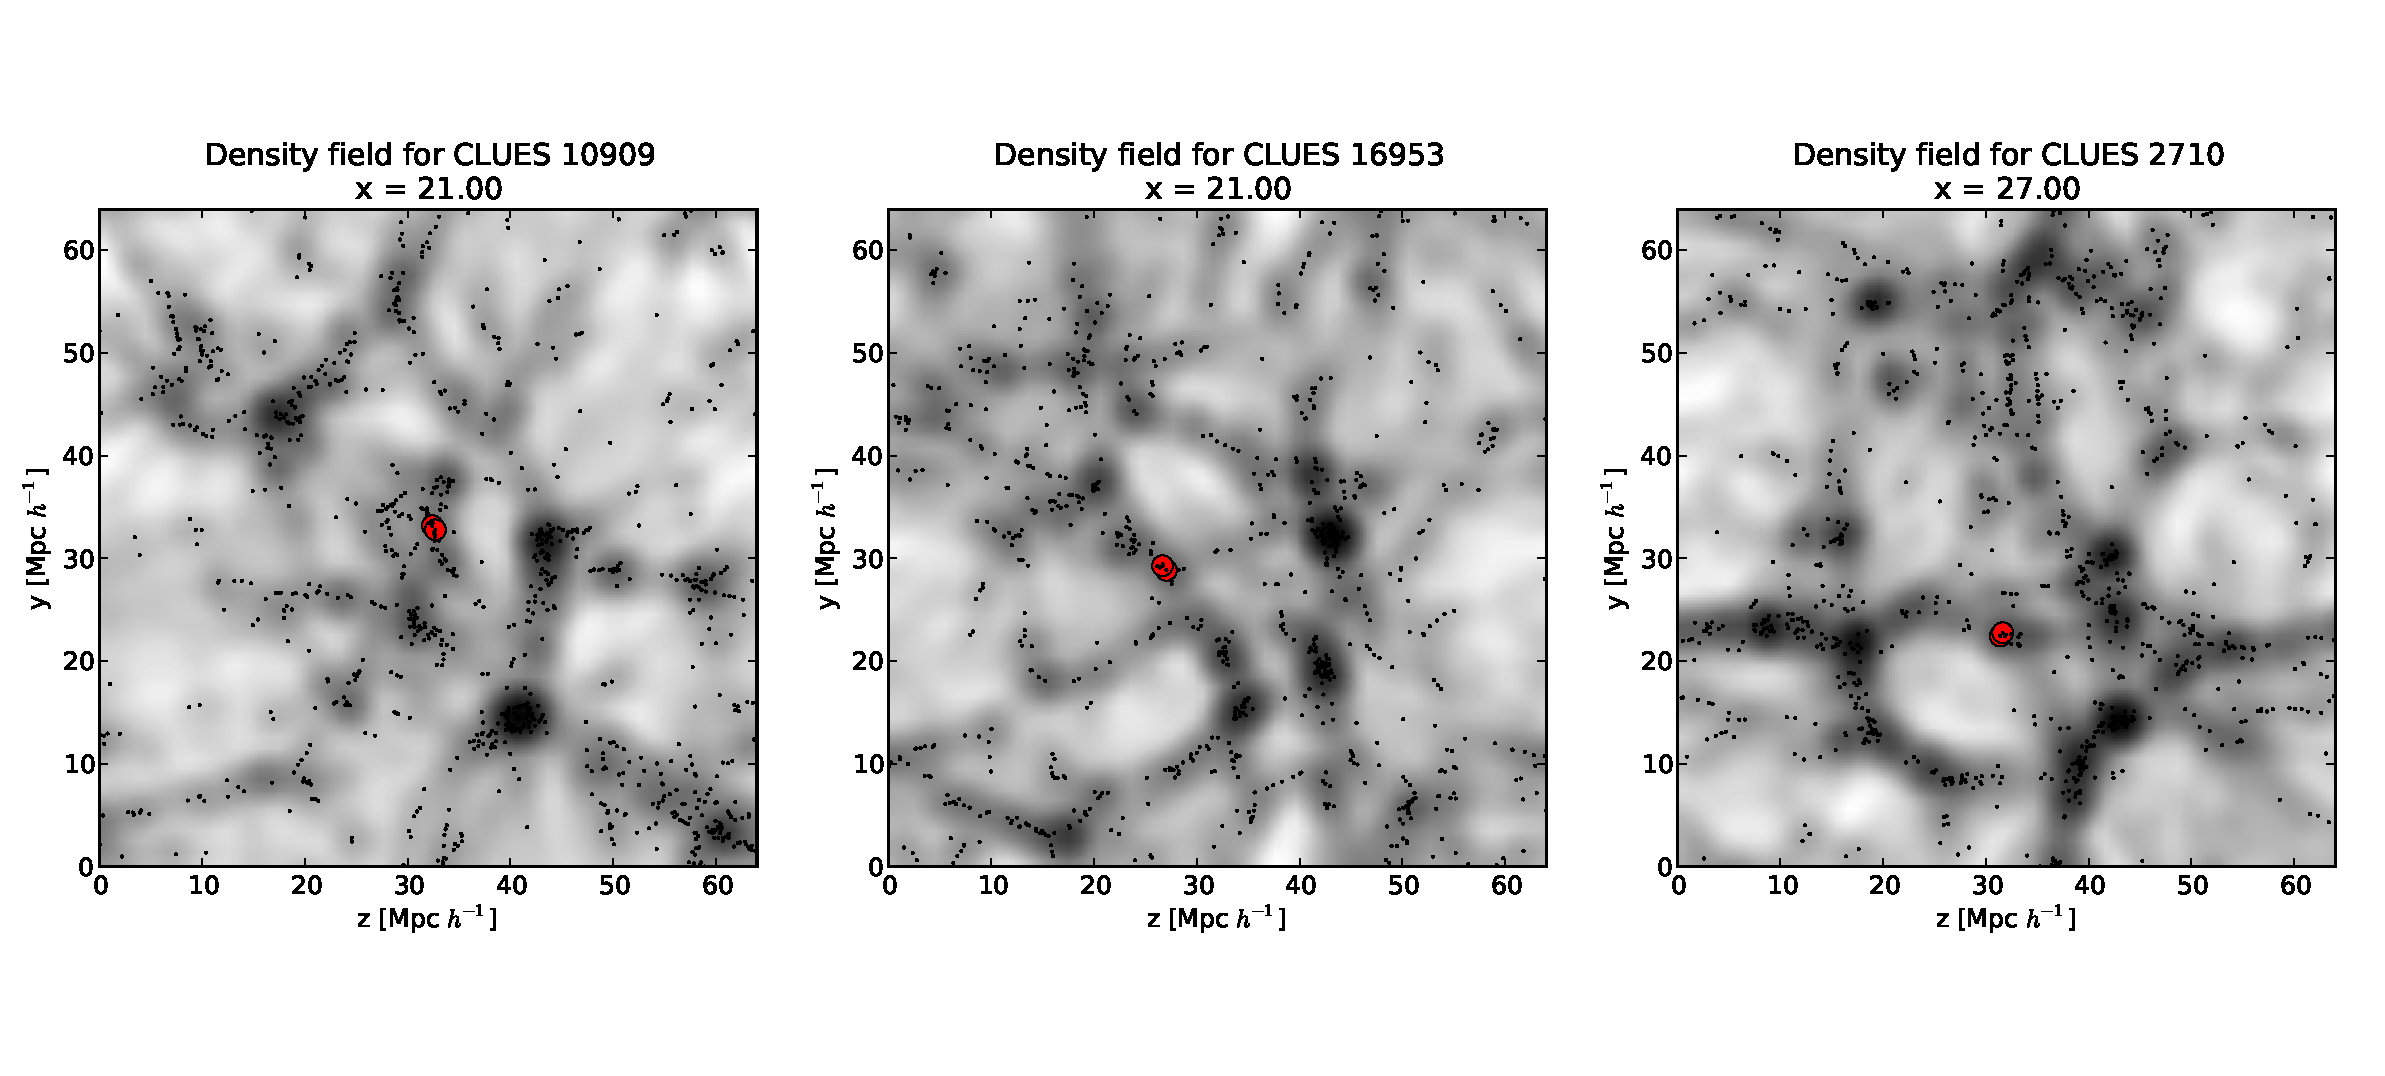
\includegraphics[trim = 5mm 5mm 0mm 5mm, clip, width=1.\textwidth]
	{./figures/CLUES_Simulations.pdf}
	
	%\end{center}
\end{columns}

\end{tcolorbox}
\end{frame}
%=========================================================================
%			CLASSIFIYING THE COSMIC WEB
\begin{frame}
\begin{tcolorbox}[colback=white!5,colframe=black!75!black,title=Classification of the Cosmic Web]\justifying
\

	\textbf{V-web Scheme}

	Dynamical classification scheme based on the shear velocity tensor 
	(Hoffman et al. 2012)
	
	\eq{Vweb}
	{\Sigma_{ij} = - \frac{ 1 }{ 2H_0 } \pr{ \derpartial{v_i}{r_j} + \derpartial{v_j}{r_i} } }

	This scheme is more adequate to classify the cosmic web at smaller 
	cosmological scales ($\gtrsim 5h^{-1}$ Mpc) compared to schemes based 
	on the density field.

\

\end{tcolorbox}
\end{frame}
%=========================================================================
%			CLASSIFIYING THE COSMIC WEB: TYPE OF REGIONS
\begin{frame}
\begin{tcolorbox}[colback=white!5,colframe=black!75!black,title=Classification of the Cosmic Web]\justifying

\

	Significant improvement by introducing a threshold parameter 
	$\lambda_{th}$ (Forero-Romero et al. 2009).

	\
	\begin{center}
	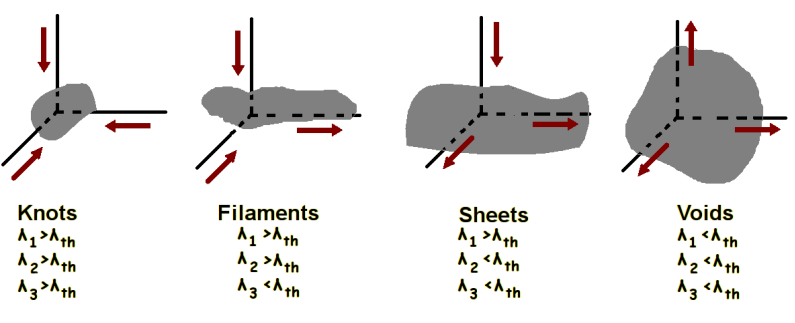
\includegraphics[trim = 0mm 0mm 0mm 0mm, clip, width=.9\textwidth]
	{./figures/EnvironmentClassification.png}
	\end{center}
	\
	
	Nevertheless, $\lambda_{th}$ is still a free parameter,	chosen 
	manually in order to reproduce the visual impression of the cosmic 
	web. 
	

\

\end{tcolorbox}
\end{frame}
%=========================================================================
%			CLASSIFIYING THE COSMIC WEB: TYPE OF REGIONS
\begin{frame}
\begin{tcolorbox}[colback=white!5,colframe=black!75!black,title=Classification of the Cosmic Web]\justifying
\

	The proposed scheme is based on the minimization of the mean density of
	vacuums, since this type of region dominates the visual appearance.

	\begin{center}
	\includegraphics[trim = 0mm 0mm 0mm 0mm, clip, width=.8\textwidth]
	{./figures/Mean_Density.pdf}
	\end{center}

\

\end{tcolorbox}
\end{frame}
%=========================================================================
%			CLASSIFIYING THE COSMIC WEB: TYPE OF REGIONS
\begin{frame}
\begin{tcolorbox}[colback=white!5,colframe=black!75!black,title=Classification of the Cosmic Web]\justifying

	\begin{center}
	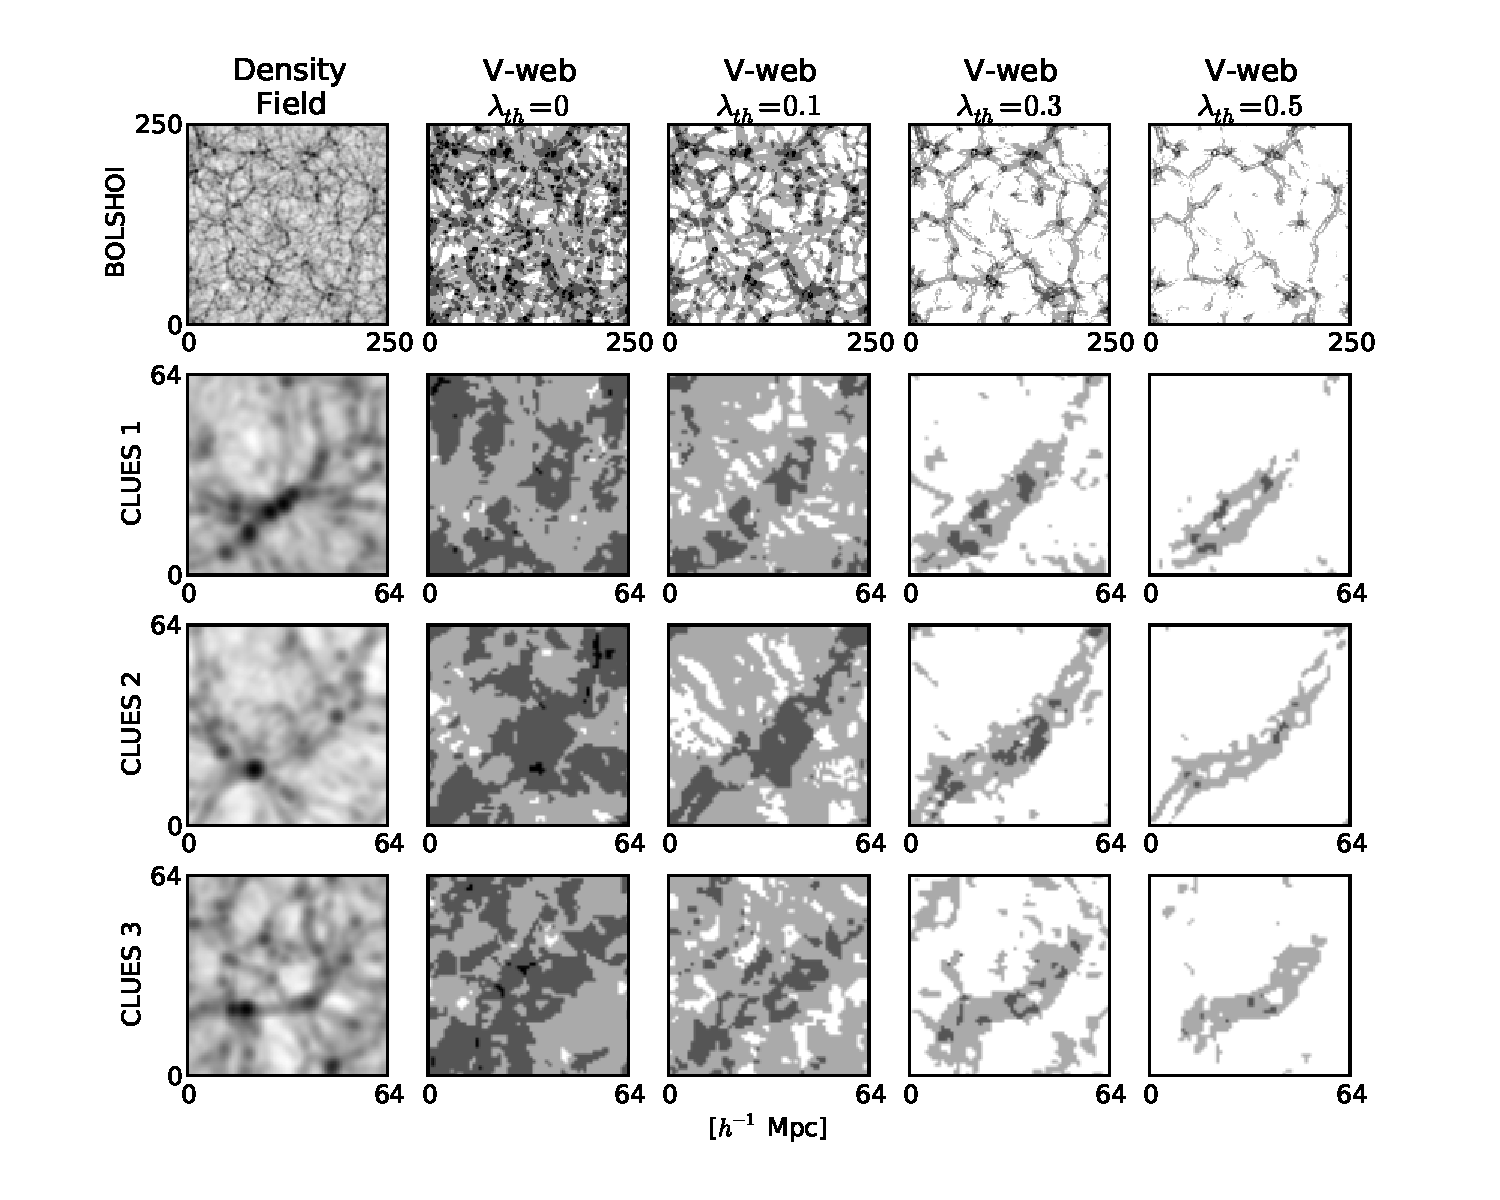
\includegraphics[trim = 5mm 5mm 5mm 5mm, clip, width=.9\textwidth]
	{./figures/Vweb_Comparison.pdf}
	\end{center}

\end{tcolorbox}
\end{frame}
%=========================================================================
%			DEFINING PAIR SAMPLES
\begin{frame}
\begin{tcolorbox}[colback=white!5,colframe=black!75!black,title=Defining the Samples]\justifying

	From FOF catalogues of dark matter halos of each simulations, it is built
	the next samples of halo pairs:

	\begin{small}	
	\begin{itemize}
	\justifying
	\color{black}
	\item \textbf{Pairs (P):} all halo pairs that satisfy the criterion to be 
	the closest neighbour to each other. \underline{Defined in Bolshoi, CLUES.}
	\item \textbf{Isolated Pairs (IP):} all halo pairs that besides, satisfy
	having a relative distance less than $0.7h^{-1}$ Mpc, negative radial 
	velocity, and being relatively isolated from more massive halos and other 
	cosmological structures. \underline{Defined in Bolshoi, CLUES.}
	\item \textbf{LG-like pairs (LG):} the three LG systems defined in each one
	of the three CLUES simulations, respectively. By construction, they are 
	embedded into a cosmological environment compatible with observations. 
	\underline{Defined in CLUES.}
	\end{itemize}
	\end{small}

\end{tcolorbox}
\end{frame}
%=========================================================================
%			DEFINING PAIR SAMPLES
\begin{frame}
\begin{tcolorbox}[colback=white!5,colframe=black!75!black,title=Defining the Samples]\justifying

	In order to obtain a faithful sample of LG-like systems in unconstrained
	simulations regarding the local environment, it is proposed the next 
	scheme.

	\begin{small}	
	\begin{itemize}
	\justifying
	\color{black}
	\item \textbf{Constructed Local Groups (CLG):} all halos pairs of the \textit{IP} 
	sample whose eigenvalues (host cell) are within the range defined by the
	LG-like systems in the constrained simulations. \underline{Defined in Bolshoi.}
	\end{itemize}

	\begin{center}
	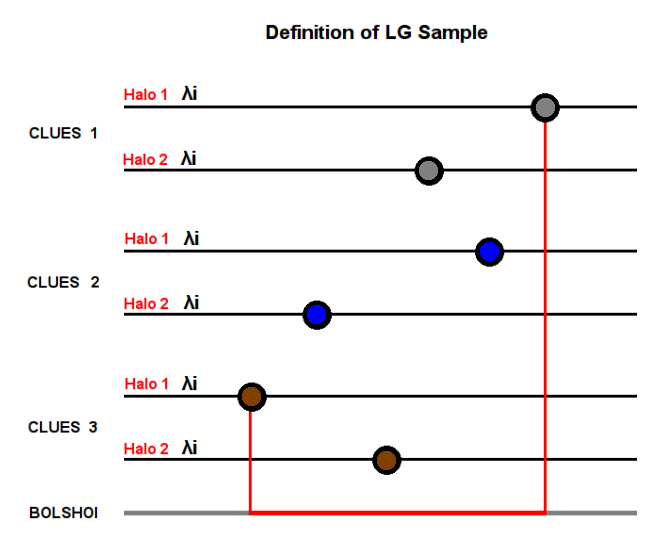
\includegraphics[trim = 5mm 5mm 5mm 15mm, clip, width=.6\textwidth]
	{./figures/LG_definition.png}
	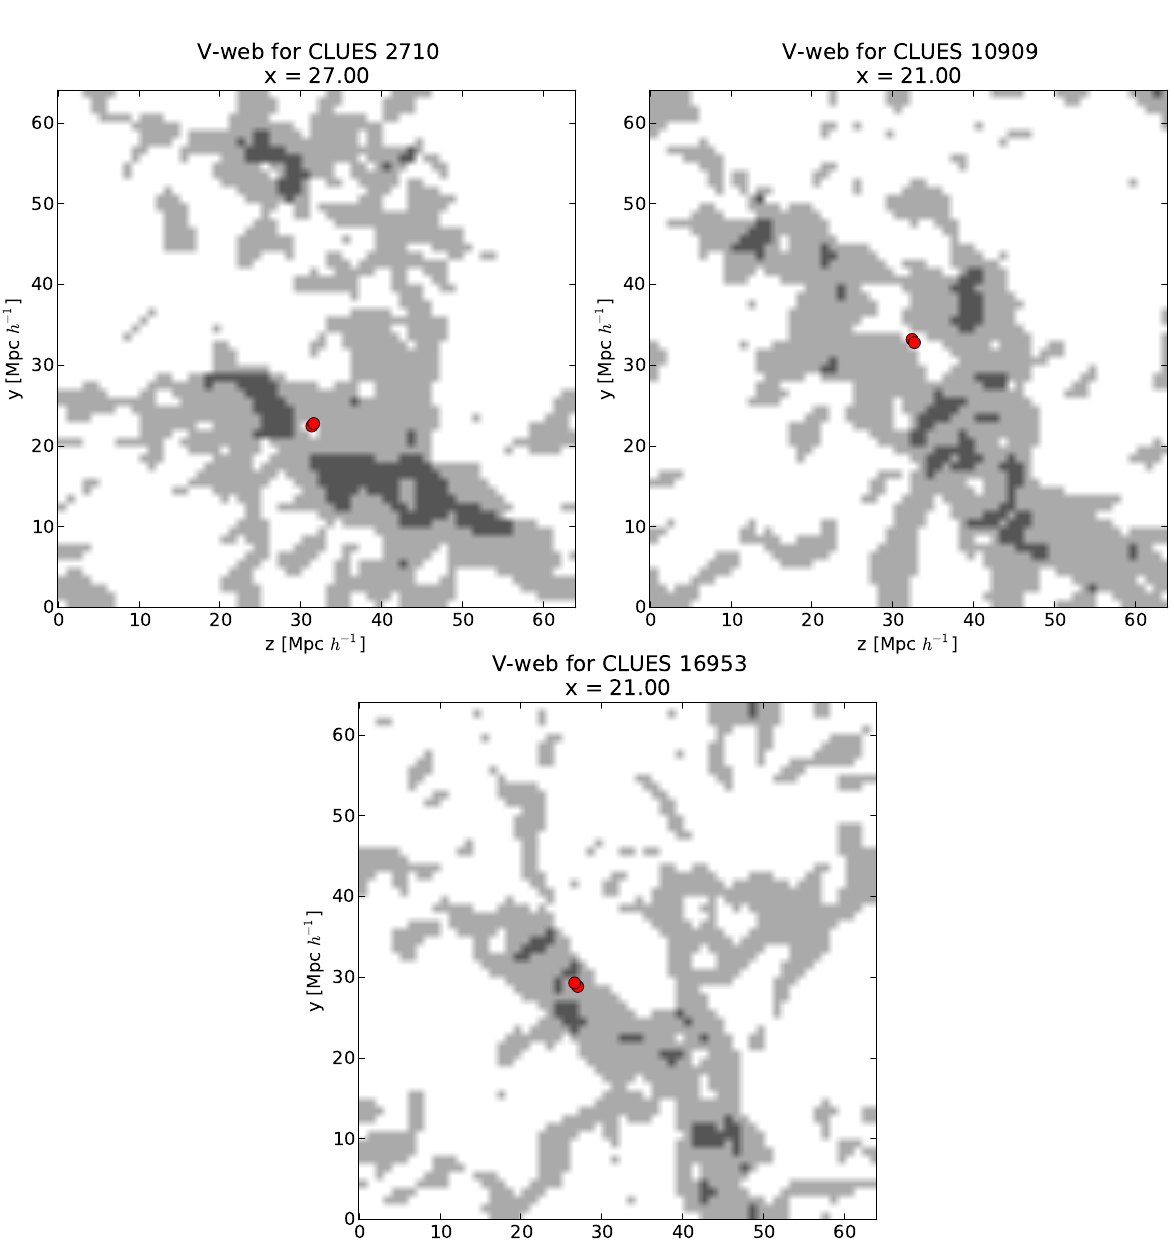
\includegraphics[trim = 0mm 0mm 0mm 0mm, clip, width=.4\textwidth]
	{./figures/LG_Environment.png}
	\end{center}
	
	\end{small}

\end{tcolorbox}
\end{frame}
%=========================================================================
%			DEFINING PAIR SAMPLES
\begin{frame}
\begin{tcolorbox}[colback=white!5,colframe=black!75!black,title=Defining the Samples]\justifying

	The size of each sample scales approximately as the volume of the 
	simulations.
	
	%Table of samples numbers
\begin{table}[htbp]
\begin{small}
  \centering
  \begin{tabular}{| c | c | c | c | c |} \hline
	\cellc{}&\cellc{}&\cellc{}&\cellc{}&\cellc{} \\  
	\cellc{\textbf{Sample}}		& 
	\cellc{\textbf{CLUES 1}}		& 
	\cellc{\textbf{CLUES 2}} 		& 
	\cellc{\textbf{CLUES 3}}		& 
	\cellc{\textbf{Bolshoi}}		 \\ 
	\cellc{}&\cellc{}&\cellc{}&\cellc{}&\cellc{} \\  \hline
	& & & & \\
	\textit{GH} 	& 56632 & 57707 & 56799  & 432000 	\\
	& & & & \\	
	\textit{IH}		& 1493 	& 1490 	& 1493	 & 88068 	\\
	& & & & \\
	\textit{P}		& 386 	& 380 	& 387	 & 23037 	\\
	& & & & \\
	\textit{IP}		& 20 	& 12 	& 18 	 & 1256 	\\
	& & & & \\
	\textit{LG}		& 1 	& 1 	& 1 	 & --		\\
	& & & & \\
	\textit{CLG}	& 1 	& 2 	& 3 	 & 30		\\ 
	& & & & \\ \hline
  \end{tabular}
  \label{tab:Samples}
\end{small}
\end{table}

Taking into account the number of systems in each simulation,
the \textit{CLG} sample in Bolshoi is a more faithful sample than 
the \textit{IP}.


\end{tcolorbox}
\end{frame}
%=========================================================================
%			COSMIC ENVIRONMENT
\begin{frame}
\begin{tcolorbox}[colback=white!5,colframe=black!75!black,title=Environment of LG-like Systems]\justifying

	The proposed method to construct the \textit{CLG} sample biases the
	host environment to low density regions, so these LG-like systems lie 
	preferentially in va\-cuums and sheets.

	\centering
	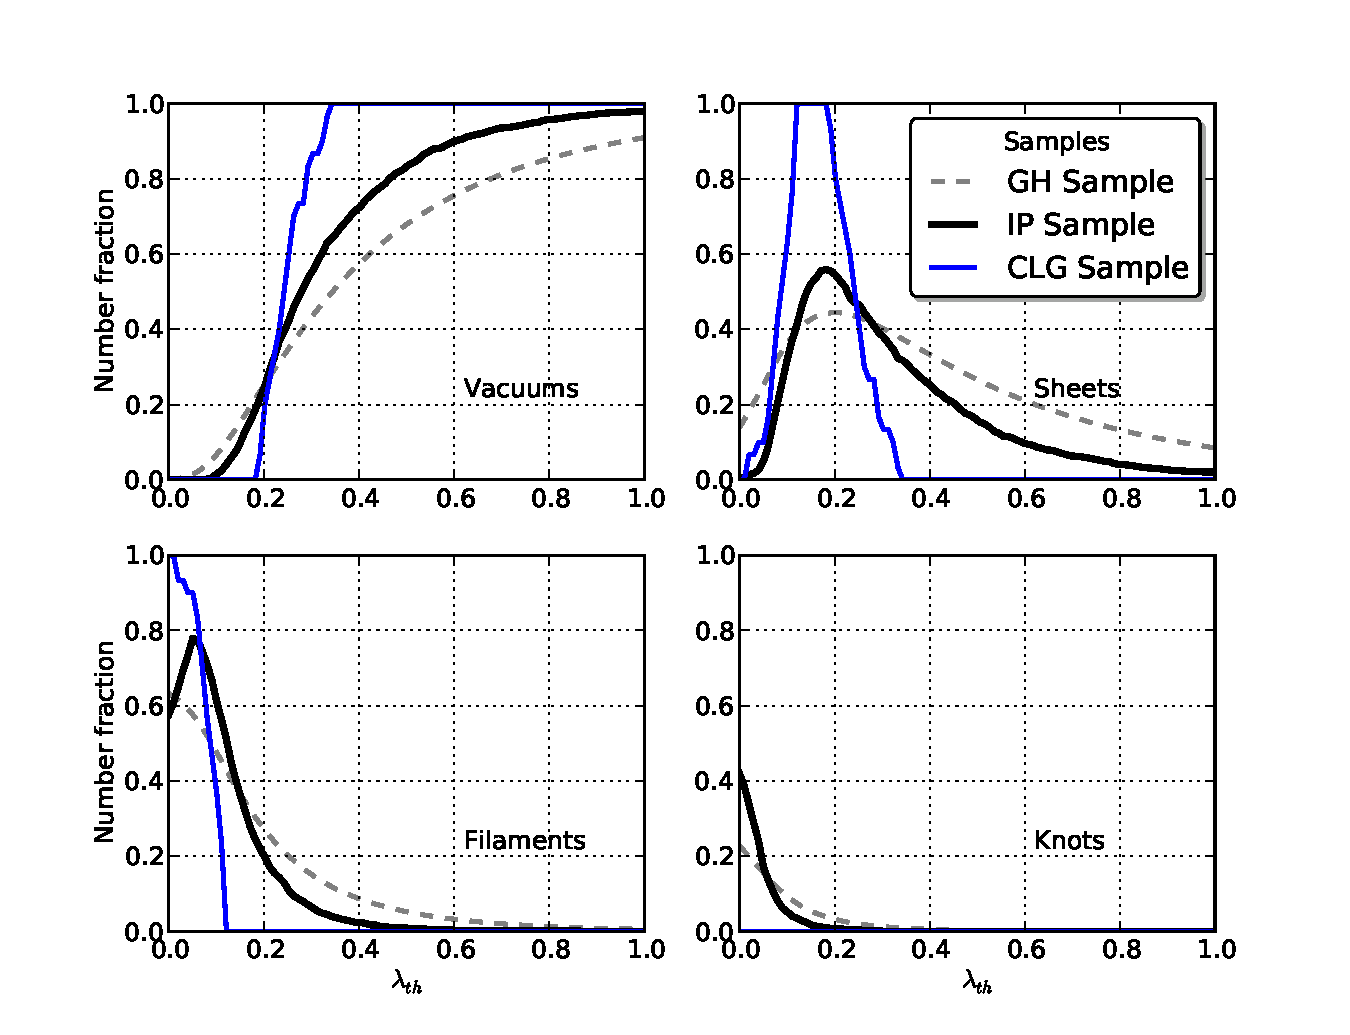
\includegraphics[trim = 5mm 5mm 5mm 5mm, clip, width=.8\textwidth]
	{./figures/CLG_Classification_Env.pdf}
	

\end{tcolorbox}
\end{frame}
%=========================================================================
%			FRACTIONAL ANISOTROPY
\begin{frame}
\begin{tcolorbox}[colback=white!5,colframe=black!75!black,title=Fractional Anisotropy]\justifying

	Another more convenient way to quantify the cosmological environment
	is the fractional anisotropy, defined as (Libeskind et al. 2013)
	
	\eq{FA}
	{ FA = \frac{1}{\sqrt{ 3 }} \sqrt{ \frac{ (\lambda_1 - \lambda_3)^2 +
	(\lambda_2 - \lambda_3)^2 + (\lambda_1 - \lambda_2)^2 }
	{ \lambda_1^2 + \lambda_2^2 + \lambda_3^2 } }  }

	This quantity quantifies the anisotropy degree of a region.
	Vacuums are biased to low FA values ($FA \sim 0$), whereas Knots to high
	values ($FA \sim 1$). Filaments and Sheets are distributed over middle
	values, even so, there are a slight tendency towards lower values for 
	Filaments and higher values for Sheets. 


\end{tcolorbox}
\end{frame}
%=========================================================================
%			COSMIC ENVIRONMENT
\begin{frame}
\begin{tcolorbox}[colback=white!5,colframe=black!75!black,title=Fractional Anisotropy]\justifying

	The distribution associated to \textit{CLG} systems is biased again
	compared with the \textit{IP} sample, confirming the preferred environment.

	\centering
	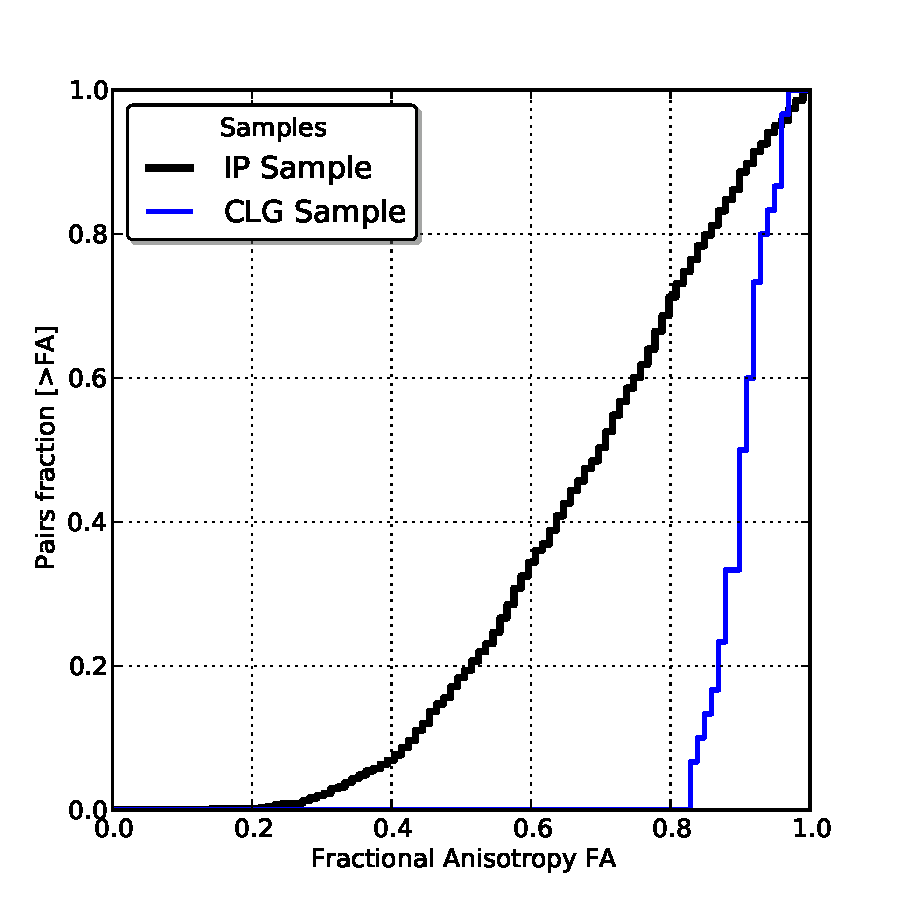
\includegraphics[trim = 5mm 5mm 5mm 5mm, clip, width=.6\textwidth]
	{./figures/CLG_FA_Hist.pdf}
	

\end{tcolorbox}
\end{frame}
%=========================================================================
%			MASS PARAMETERS
\begin{frame}
\begin{tcolorbox}[colback=white!5,colframe=black!75!black,title=Mass of LG-like systems]\justifying

	It has been found an environmental bias with respect to the total mass
	of \textit{CLG} systems, but not for the mass ratio.

	\centering
	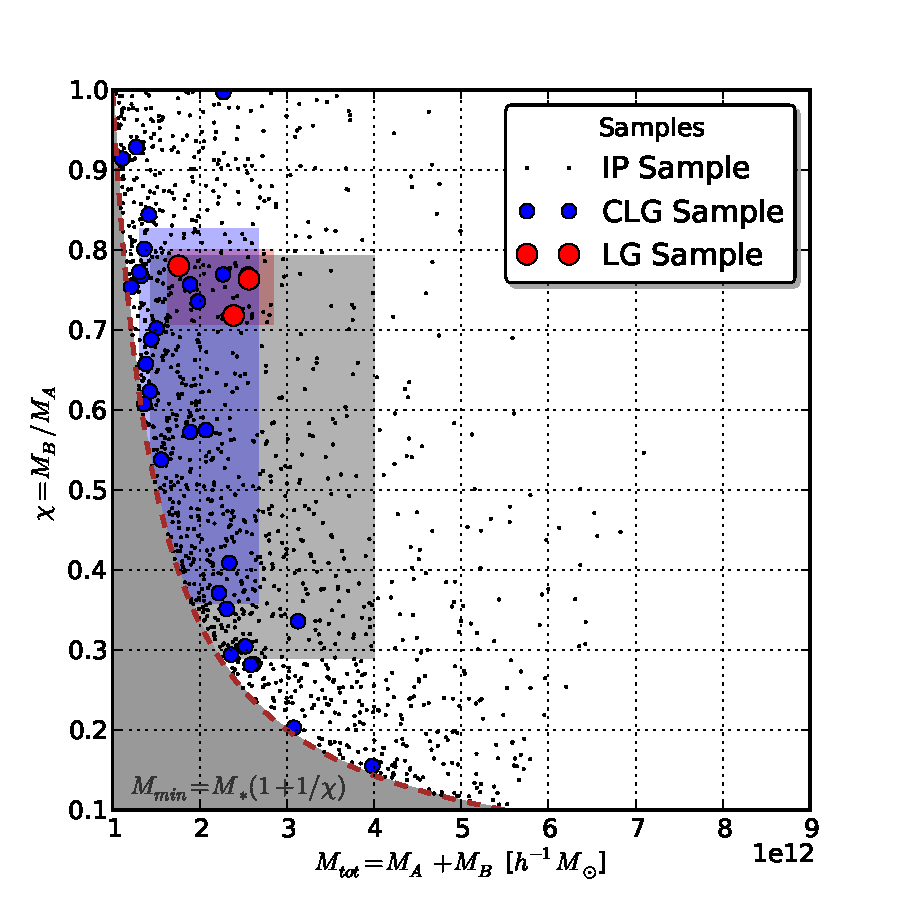
\includegraphics[trim = 5mm 5mm 5mm 5mm, clip, width=.6\textwidth]
	{./figures/IP_Mass_vs_Ratio.pdf}
	

\end{tcolorbox}
\end{frame}
%=========================================================================
%			ENERGY PARAMETERS
\begin{frame}
\begin{tcolorbox}[colback=white!5,colframe=black!75!black,title=Energy and Angular Momentum of LG-like systems]\justifying

	Considering each pair system as a isolated system, it is calculated the
	specific energy and the specific orbital angular momentum. 

	\centering
	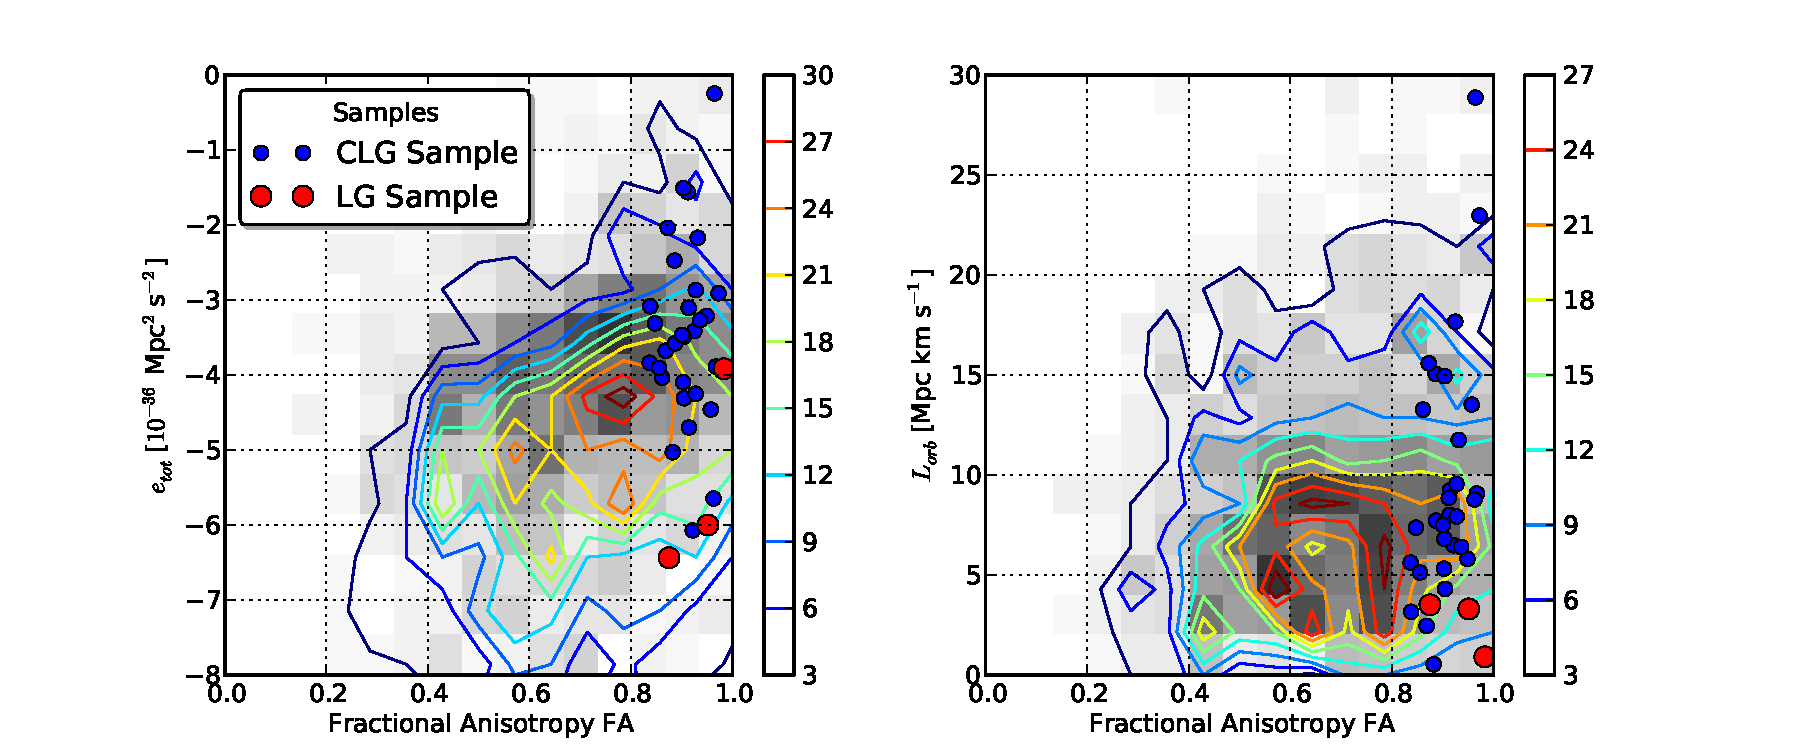
\includegraphics[trim = 5mm 0mm 5mm 5mm, clip, width=1.\textwidth]
	{./figures/CLG_FA_E-L.pdf}
	
	\justifying
	It can be noticed a bias for the energy but not for the angular momentum.
	Higher values of energy are more abundant in high anisotropic regions, whereas
	lower values are distributed over middle anisotropic zones.

\end{tcolorbox}
\end{frame}
%=========================================================================
%			ALIGNMENT
\begin{frame}
\begin{tcolorbox}[colback=white!5,colframe=black!75!black,title=Alignment of LG-like systems]\justifying

	Finally, it is calculated the alignment of the angular momentum with
	each one of the eigenvector of the V-web.
	
	\
	
	\centering
	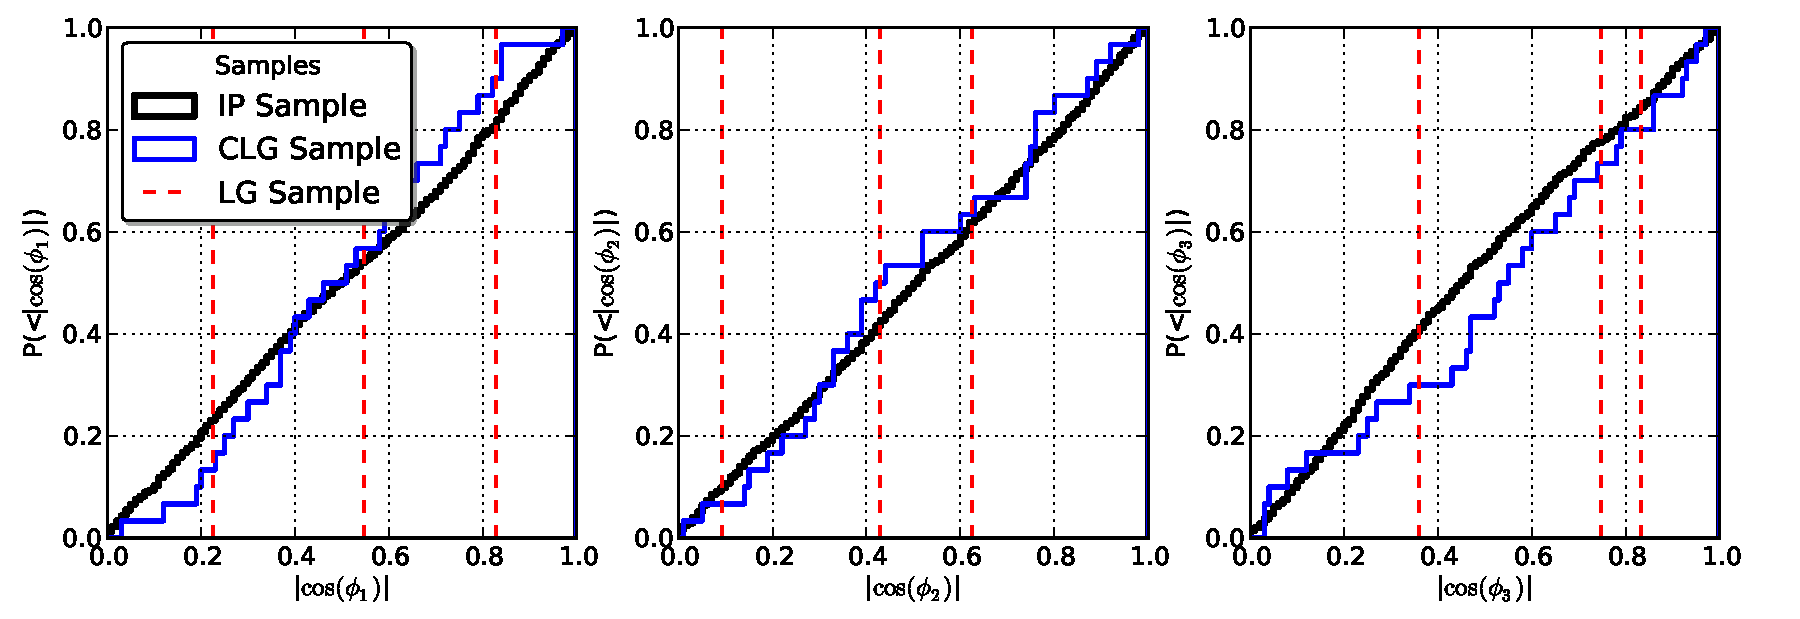
\includegraphics[trim = 0mm 0mm 0mm 0mm, clip, width=1.\textwidth]
	{./figures/CLG_Alineation.pdf}
	
	\	
			
	\justifying
	No preferred alignments have been found, although further data are necessary
	to conclude.

\end{tcolorbox}
\end{frame}
%=========================================================================
%			CONCLUSIONS
\begin{frame}
\begin{tcolorbox}[colback=white!5,colframe=black!75!black,title=Conclusions]\justifying

	\begin{itemize}
	\color{black}	
	\item The proposed method to set the threshold parameter of the V-web 
	scheme reproduces properly the visual appearance of the cosmic web, and 
	works fine for both simulations, obtaining similar values.
	
	\item The numbers of samples in each simulation scales approximately as
	their volumes.	
	
	\item The proposed method to construct LG-like systems in the Bolshoi
	simulation biases the environment, being preferred high anisotropic and
	low density regions, like sheets and vacuums.
	
	\item The criterion to select CLG systems according to the environment of
	the LG sample in CLUES, biases the total mass distribution, but not the 
	mass ratio.
	
	\item There is an environmental bias in the specific energy of \textit{IP}
	systems, but not for the angular momentum. Furthermore, any preferred
	alignment has been found for the orbital plane.
	
	\end{itemize}

\end{tcolorbox}
\end{frame}
%=========================================================================
%			FURTHER WORK
\begin{frame}
\begin{tcolorbox}[colback=white!5,colframe=black!75!black,title=Further Work]\justifying

	\begin{itemize}
	\color{black}	
	\item Look for other possible correlations for other physical properties.
	\item Compare with classification schemes based on the density field.
	\item Use BDM catalogues instead of FOF.
	\item Look for possible effects of near voids (large-scale voids).
	\item Use observational constrains in a direct way instead of using 
	constrained simulations.
	\end{itemize}

\end{tcolorbox}
\end{frame}
%=========================================================================
%			THANK YOU!
\begin{frame}
\begin{tcolorbox}[colback=white!5,colframe=black!75!black,title=And finally]\justifying

	\begin{huge}
	\begin{center}
	Thank you!
	\end{center}
	\end{huge}

	\tcblower

	Further information and the corresponding bibliography can be found in 
	the next github repository

	\url{https://github.com/sbustamante/Thesis}

\end{tcolorbox}
\end{frame}
%=========================================================================


\end{document}